\chapter{Introducción}

\textbf{EC2}, que es la contracción de las siglas en inglés \textit{Elastic Compute Cloud}, es la parte central de AWS que tiene que ver con la computación, donde podremos crear máquinas virtuales y gestionar todo lo relacionado con ellas.

Dentro del apartado EC2 podremos crear las máquinas virtuales (llamadas \textbf{instancias}) donde después alojaremos o desplegaremos los servicios que nos interese. También podremos crear backups de ellas, crear imágenes para levantar instancias de manera más rápida, securizarlas...

\chapter{Instancias}

Una instancia es cómo llama AWS a una máquina virtual, por lo que los conocimientos previos que tengamos sobre máquinas virtuales se pueden asociar una instancia EC2 de AWS. Podemos realizar distintas acciones sobre las instancias que ya tengamos creadas.

Antes de crear una instancia debemos entender distintos apartados ya que a la hora de lanzar una instancia (crearla), se nos pedirá que elijamos entre distintas opciones disponibles que hay. Es similar a lo que sucede cuando creamos una máquina virtual con Virtualbox.

\section{Tipos de instancia}

El tipo de instancia hace referencia a parte del hardware que va a tener disponible la máquina virtual al realizar el despliegue. Existe una infinidad de tipos de instancias, y es por eso que conviene leer la \href{https://docs.aws.amazon.com/AWSEC2/latest/UserGuide/instance-types.html#AvailableInstanceTypes}{documentación oficial} ya que en ella se detalla mucho más para qué sirve cada tipo de arquitectura.

Los nombres de las instancias siguen un convenio que viene explicado en la documentación oficial.

\begin{center}
	\includesvg[]{ec2_instance_name_convention.svg}
\end{center}

Dado que el número de tipos de instancias actualmente es mayor que 700, puede resultar complejo saber exáctamente de primera mano cuál debemos elegir. Por otro lado, en el listado que podemos ver en el panel de EC2, nos aparece la información que simple vista nos puede dar una idea de cómo es el tipo de instancia.

\infobox{\textbf{Para asegurar que se adecúa a nuestras necesidades, es mejor confirmar el tipo de instancia que necesitamos mirando la \href{https://docs.aws.amazon.com/AWSEC2/latest/UserGuide/instance-types.html}{documentación oficial}.}}

\begin{center}
	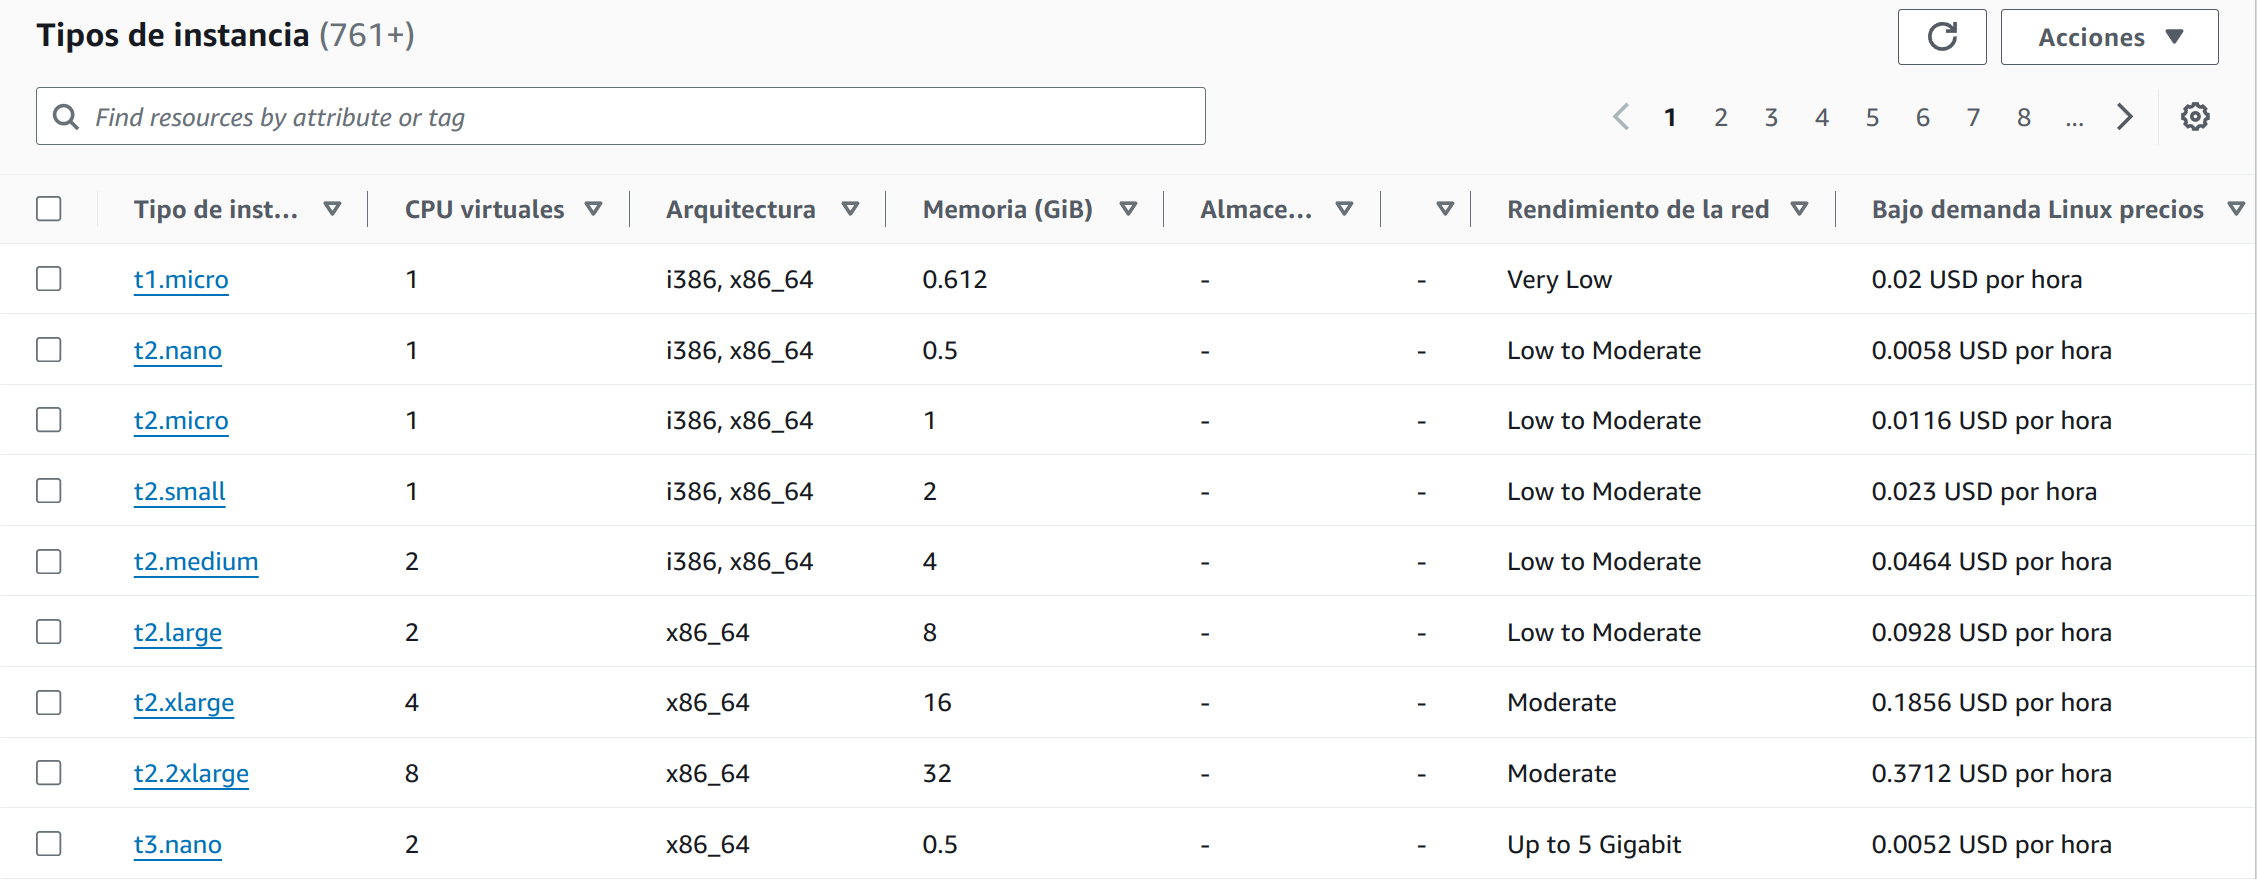
\includegraphics[frame,width=0.8\linewidth]{ec2_instance_types.png}
\end{center}

Los valores que podemos identificar a simple vista son:

\begin{itemize}
	\item \textbf{CPU virtuales}: El número de cores virtuales que el procesador virtual tendrá a su disposición. Dependiendo de nuestras necesidades de cómputo y procesamiento, deberemos elegir un número que se adecúe al rendimiento que esperamos. Actualmente podemos elegir tipos de instancias que tengan entre 1 y 448 CPUs.
	
	\item \textbf{Arquitectura}: Es el tipo de arquitectura del procesador con el que se desplegará la máquina virtual. Entre las arquitecturas que podemos elegir están:
	\begin{itemize}
		\item \textbf{i386}: Arquitectura clásica de equipos de 32 bits.
		\item \textbf{x86\_64}: Arquitectura actual para equipos y servidores.
		\item \textbf{x86\_64\_mac}: Arquitectura utilizada por los equipos Mac con procesadores Intel.
		\item \textbf{arm64}: Arquitectura ARM de 64 bits.
		\item \textbf{arm64\_mac}: Arquitectura ARM de los nuevos procesadores M* de Apple.
	\end{itemize}
	
	\item \textbf{Memoria}: Tamaño de la memoria RAM medido en GiB.
	
	\item \textbf{Rendimiento de la red}: Velocidad de la conexión de red que tendrá la instancia.
	
	\item \textbf{Precio de la instancia}: El coste de la instancia cuando está en funcionamiento se mide en doláres americanos (USD) por hora. El precio varía si el sistema operativo que va a correr la instancia es Linux o Windows, y por supuesto del resto de componentes virtuales.
	
\end{itemize}

\warnbox{\textbf{Se puede cambiar el tipo de instancia, pero para ello se debe parar la instancia}. }


\section{Imágenes AMI}

Una imagen AMI (\textit{Amazon Machine Image})es una plantilla que contiene la configuración del software (el sistema operativo, los servicios y aplicaciones) que son necesarias para correr dentro de nuestra instancia. Existen imágenes AMI públicas creadas por proveedores de software verificados entre las que podremos elegir. 

Hay un catálogo de AMI entre las que podemos elegir:

\begin{itemize}
	\item \textbf{Quickstart AMIs}: Imágenes que normalmente suelen ser el sistema operativo con el mínimo software necesario para hacerlo funcionar. Para correr el resto de servicios, necesitaremos instalar lo que necesitemos.
	
	\item \textbf{Mis AMI}: Podemos crear nuestras propias imágenes para poder reusarlas cuando queramos.
	
	\item \textbf{AMI de AWS Marketplace}: Son imágenes creadas por empresas que pueden contener servicios de alto rendimiento, y \textbf{que en muchos casos pueden ser de pago (por licencia o uso)}.
	
	\item \textbf{AMI de la comunidad}: Imágenes que pueden ser creadas por proveedores oficiales o por comunidades que crean imágenes con software específico.
\end{itemize}

\begin{center}
	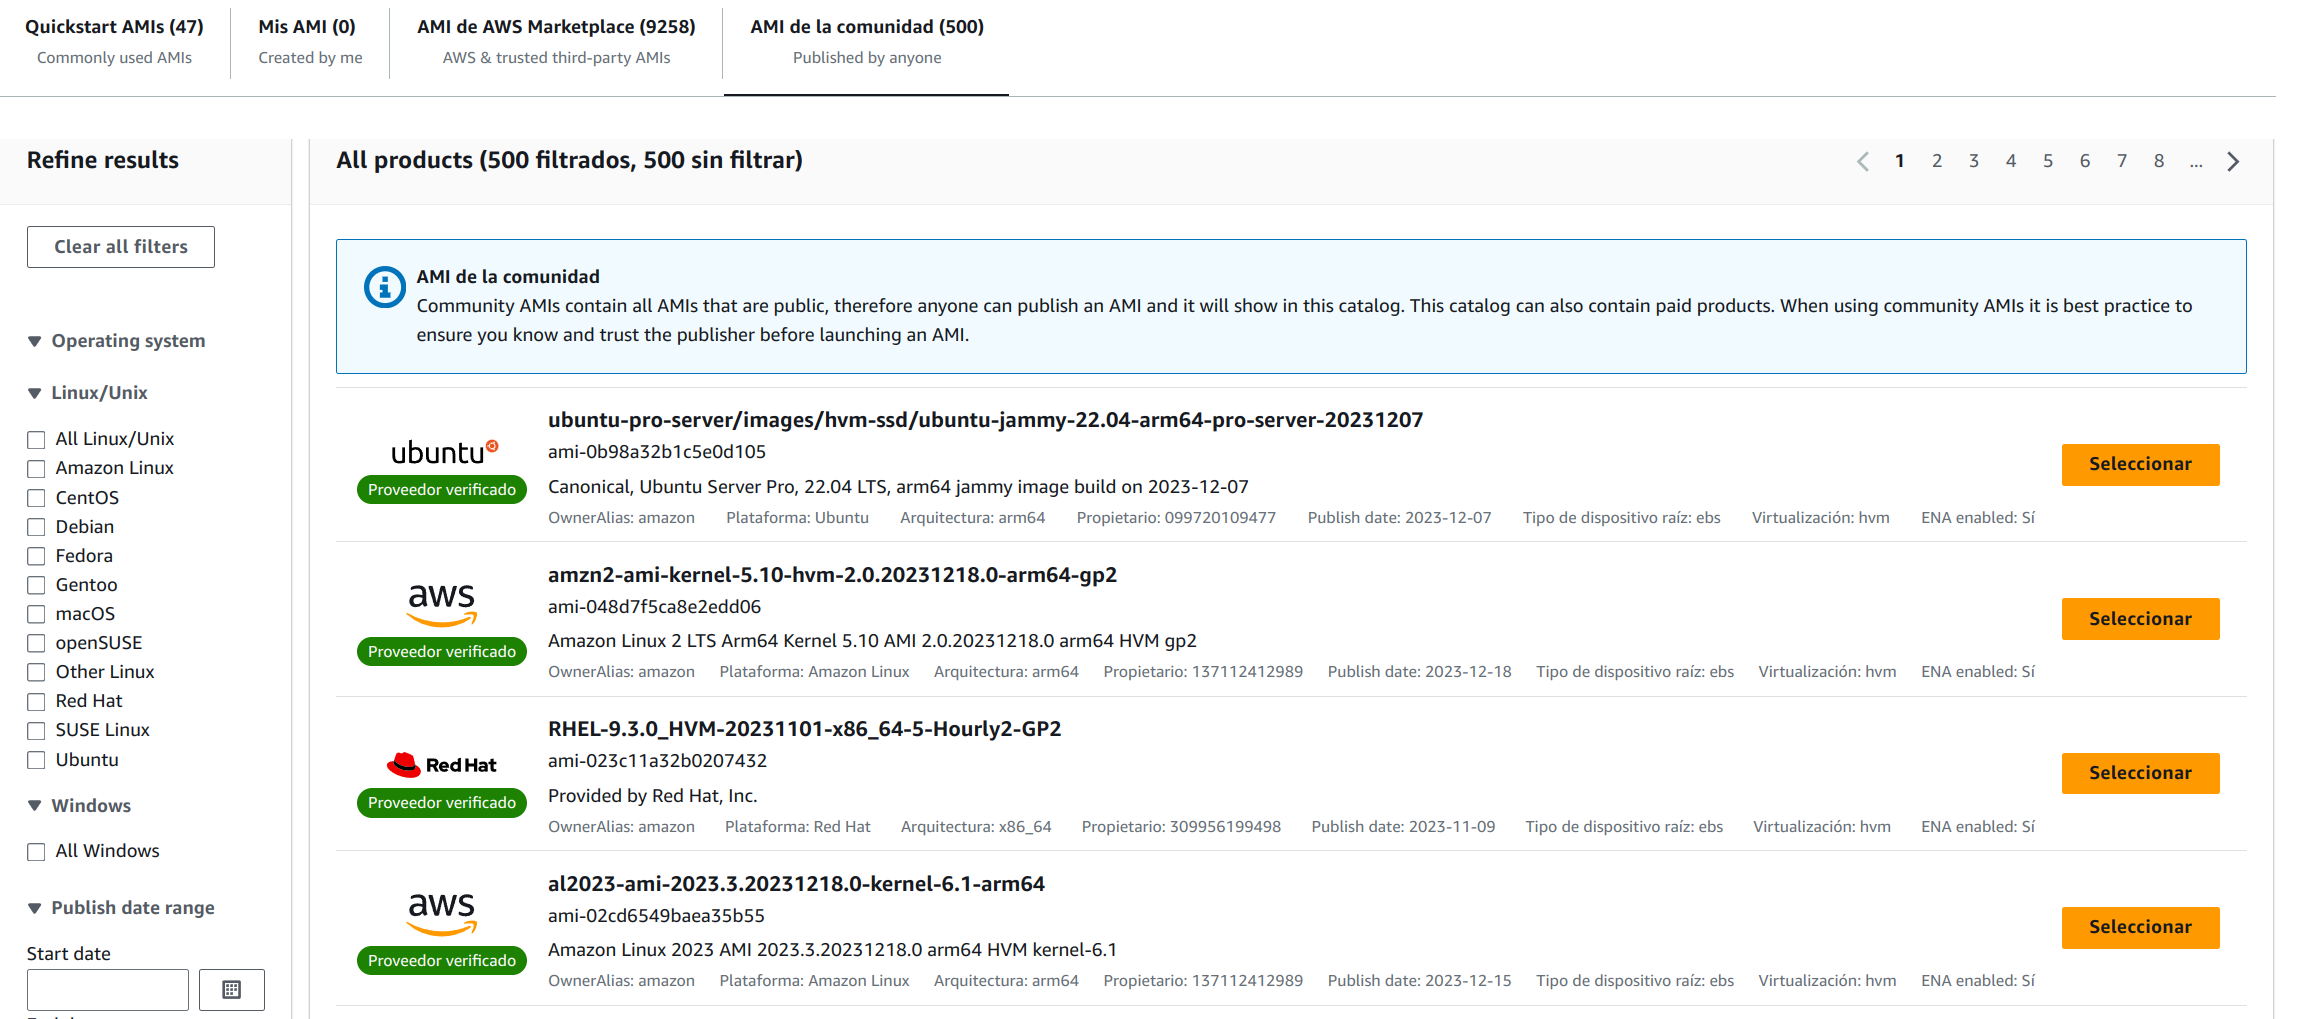
\includegraphics[frame,width=0.9\linewidth]{ec2_ami_catalogue.png}
\end{center}




\infobox{\textbf{Podemos crear nuestras propias imágenes para poder reusarlas cuando queramos.}}

Para empezar, podemos crear nuestra instancia con una imagen AMI de un proveedor oficial, para posteriormente utilizarla como base para crear una AMI propia.


\section{Crear una instancia}

A continuación se va a explicar cómo crear una instancia de tipo Linux teniendo en cuenta todas las posibles opciones que podemos elegir. Para crearla haremos click en 
\includegraphics[height=0.8\baselineskip]{ec2_instance_create.png} y seguiremos las indicaciones para adecuarla a nuestras necesidades.

Las respuestas que debemos contestar y tener en cuenta son:

\begin{itemize}
	\item \textbf{Nombre y etiquetas}: Es el nombre que le vamos a dar a la instancia (que debería ser un nombre significativo), y posibles etiquetas para identificarla.
	
	\item \textbf{Application and OS Images (Amazon Machine Image)}: Imagen AMI que queremos desplegar en la instancia.
	
	\item \textbf{Arquitectura}: Arquitectura del procesador.
	
	\item \textbf{Tipo de instancia}: El tipo de instancia que queremos desplegar para las necesidades que tenemos.
	
	\item \textbf{Par de claves (inicio de sesión)}: El par de claves asimétricas (\textbf{pública-privada}) que vamos a utilizar para realizar la conexión a la instancia. Más adelante explicaremos cómo acceder a la instancia. 
	
	\warnbox{\textbf{Debemos elegir el par de claves “vockey” para poder acceder a la instancia.}}
	
	\item \textbf{Configuraciones de red}: Ajustar las configuraciones de red. Por defecto podemos elegir el \textbf{grupo de seguridad} que queremos asignar a la instancia. Como opciones avanzadas, podemos desactivar el tener IP pública o asignar la instancia a una subred.

	\errorbox{\textbf{La IP pública que se asigna no es “eterna”. Cuando se apague la instancia y se vuelva a levantar obtendrá otra IP pública.}}
	
	\item \textbf{Configurar almacenamiento}: El disco duro principal de la instancia.
	
	\item \textbf{Opciones avanzadas}: Distintas opciones de configuraciones que podemos modificar o de hardware que podemos habilitar.
\end{itemize}

A la derecha del asistente tenemos tenemos un resumen en el que nos aparece las distintas opciones seleccionadas. En este resumen podemos elegir el número de instancias que nos interese crear, por si queremos más de una.

Una vez le damos a “Lanzar instancia” la instancia se creará y empezará el despliegue. Desde el panel de instancias, si seleccionamos la instancia recién creada veremos todos los detalles de la misma:

\begin{center}
	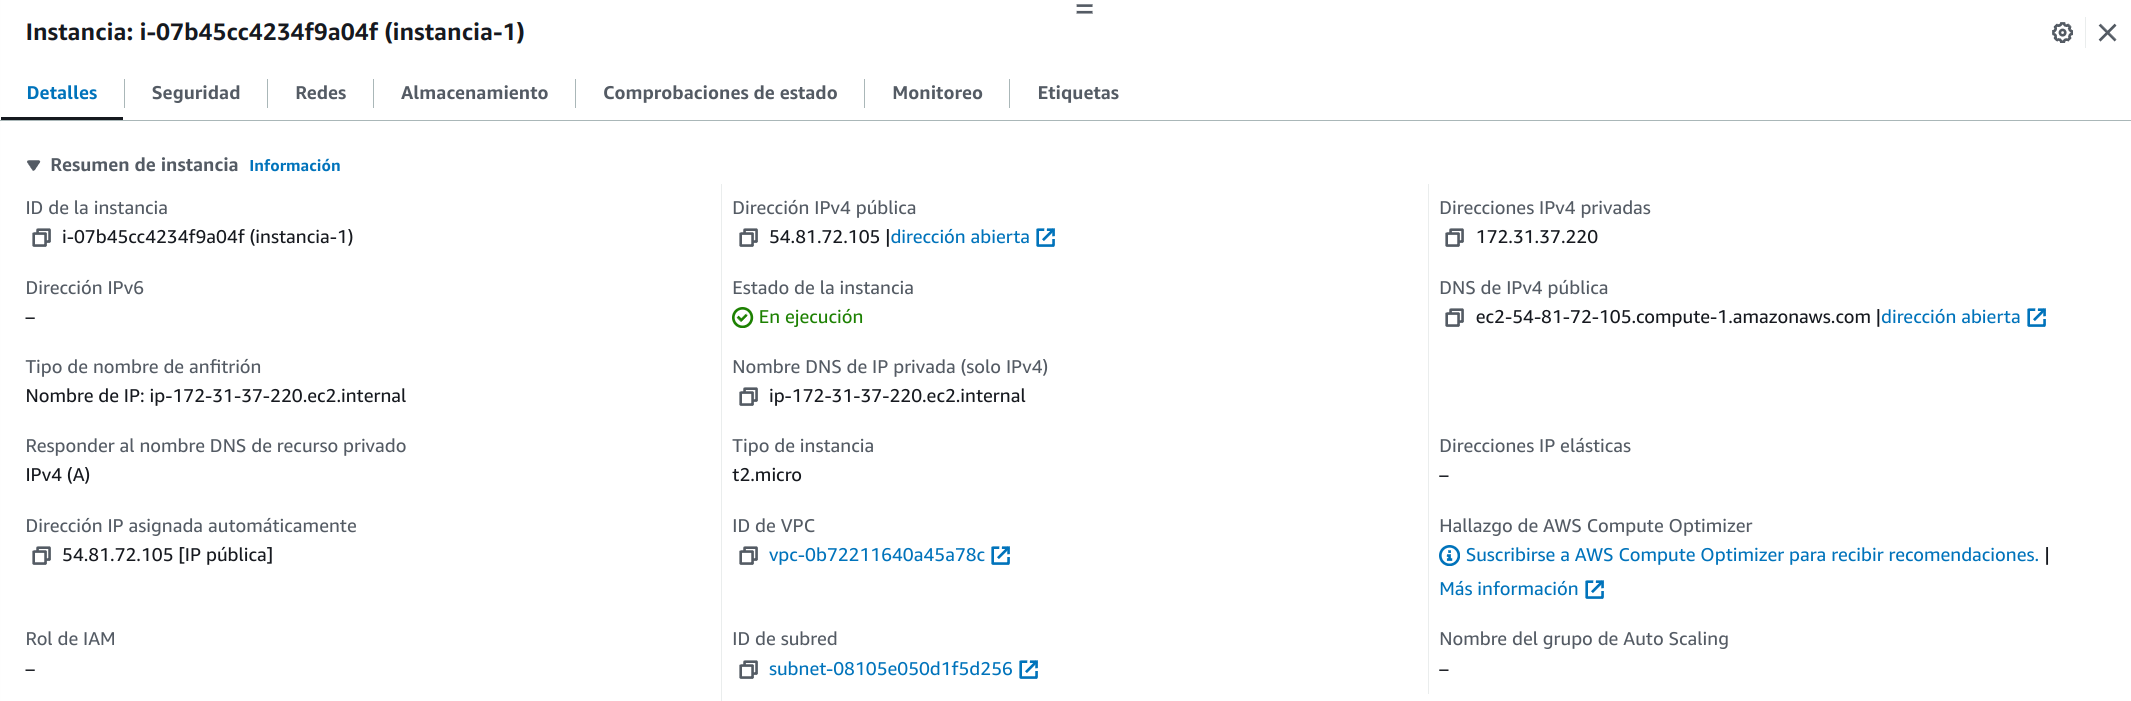
\includegraphics[frame,width=0.9\linewidth]{ec2_instance_info.png}
\end{center}

Tal como se puede ver, la información de la instancia está separada en distintas pestañas y en cada una de ellas nos aparecerá mucha información sobre la misma. Parte de esta información será la necesaria para poder acceder a la instancia por SSH.


\section{Acceder a una instancia}

Para acceder a una instancia desplegada tenemos distintas opciones que podemos visualizar desde el botón 
\includegraphics[height=0.8\baselineskip]{ec2_instance_connect.png} cuando esté la instancia seleccionada. Entre las opciones, vamos a destacar dos:

\begin{itemize}
	\item \textbf{Conexión de la instancia EC2}: Es el método más sencillo para acceder a una instancia a través de SSH, ya que vamos a poder realizar la conexión a través del propio navegador web. Esto, por otro lado, no nos va a permitir hacer uso de todas las características que tiene una terminal real.
	
	\item \textbf{Cliente SSH}: Al igual que sucede al conectarnos a una máquina virtual normal,  poder acceder a la instancia a través de un cliente SSH de consola. Para ello, necesitamos conocer:
	\begin{itemize}
		\item \textbf{Nombre de usuario}: Dependiendo de la AMI que hayamos desplegado, el usuario de conexión será distinto. Por ejemplo, para instancias Ubuntu el usuario es “\textbf{ubuntu}”; para instancias Debian el usuario es “\textbf{admin}”; para instancias Amazon Linux, el usuario es “\textbf{ec2-user}”. \textbf{Estos usuarios tienen la posibilidad de convertirse en “root” usando el comando sudo}.

		\infobox{\textbf{Dependiendo de la AMI elegida, el usuario de acceso será distinto.}}

		\item \textbf{DNS público / IP pública}: Lógicamente, para poder acceder a la instancia, debemos conocer cuál es su IP pública. Dado que la IP va a cambiar, Amazon genera un nombre de DNS público que siempre se mantiene y que apuntará a la IP pública que la instancia tiene en todo momento.
		
		\warnbox{\textbf{Es recomendable usar la dirección DNS pública al realizar la conexión.}}
		
		\item \textbf{Clave privada de acceso}: El usuario por defecto de la instancia no cuenta con contraseña, por lo que para acceder necesitamos hacer uso de una autenticación basada en \textbf{clave asimétrica} (conocidas también como “\textbf{clave pública-privada}”).
		
		\warnbox{\textbf{Para poder acceder a la instancia es necesario usar claves asimétricas.}}
		
	\end{itemize}
\end{itemize}


\subsection{Obtener clave privada}

Tal como se ha dicho previamente, para poder acceder a las instancias recién creadas debemos hacer uso del sistema de claves asimétricas, ya que es el método más seguro de conexión, y así no dependemos de contraseñas.

Al crear el laboratorio se nos ha creado un par de claves llamadas “\textbf{vockey}”, que sólo podemos descargar desde el panel del curso, en el apartado “\faInfo  \textbf{ AWS Details}”, dándole al botón 
\includegraphics[height=0.8\baselineskip]{ec2_download_pem.png}, que nos descargará un fichero llamado \textbf{labuser.pem}.

\textbf{Este fichero de clave debe tener permisos especiales}. Los ficheros de tipo Linux son que sólo debe tener permisos de lectura para el usuario, dejando el resto de permisos sin asignar. Por lo tanto, en formato binario, \textbf{400}. Para ello debemos hacer:

\begin{mycode}{Cambios de permisos en el fichero}{console}{}
ruben@vega:~$ chmod 400 labuser.pem
\end{mycode}

Para realizar la conexión a la instancia, y teniendo en cuenta los datos comentados previamente, el acceso se realizará utilizando el siguiente comando, sustituyendo los datos correspondientes por los correspondientes para la instancia:

\begin{mycode}{Conexión a una instancia mediante cliente SSH}{console}{{\footnotesize }}
ruben@vega:~$ ssh -i labsuser.pem admin@ec2-52-70-81-181.compute-1.amazonaws.com
admin@ip-172-31-32-168:~$ sudo su
root@ip-172-31-32-168:/home/admin#
\end{mycode}

De esta manera, ya estaremos dentro de la instancia desplegada en AWS, y podremos empezar a desplegar el servicio que nos interese.


\subsection{Crear nuevo par de claves}
En entornos profesionales \textbf{es habitual crear distintas par de claves para cada proyecto, o incluso para cada instancia}, ya que de conseguir una (o en sistemas basados en contraseñas), se obtendría acceso a un gran número de instancias, \textbf{lo que es un fallo de seguridad de extrema gravedad}.

\errorbox{\textbf{En entornos profesionales nunca se debería reutilizar claves, y menos entre distintos proyectos.}}

Si queremos crear un nuevo par de claves lo podemos realizar desde el menú lateal, en el apartado: “\textbf{Red y seguridad → Pares de claves}”. Ahí podremos hacer click sobre el icono 
\includegraphics[height=0.8\baselineskip]{ec2_new_key.png}, que nos redirigirá a un formulario donde crear las nuevas claves.

\begin{center}
	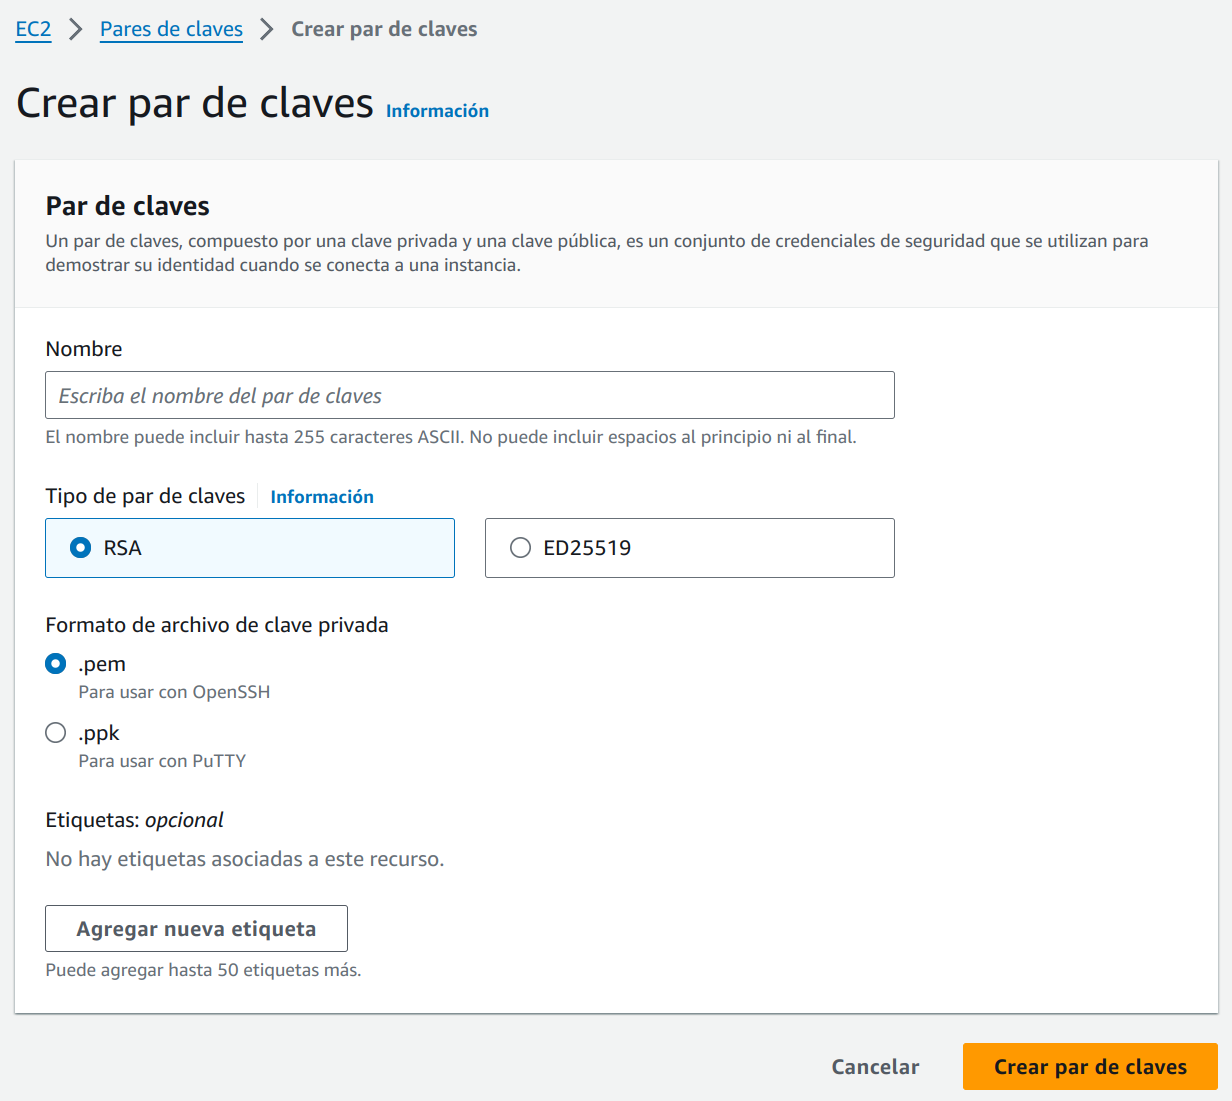
\includegraphics[frame,width=0.8\linewidth]{ec2_new_key2.png}
\end{center}

Una vez rellenado los datos, al darle al botón de crear, se nos descargará el fichero \textbf{que nunca más podremos volver a descargar}, por lo que deberemos guardarla a buen recaudo. A partir de ahora, al crear una nueva instancia, podremos hacer uso de esta nueva clave para el poder realizar el acceso con ella.

\errorbox{\textbf{¡Cuidado con el certificado descargado! No lo podremos volver a descargar.}}


\chapter{Direcciones IP elásticas}

Una IP elástica es una \textbf{IPv4 de direccionamiento público} que podemos asignar a una instancia EC2 (o a un interfaz de red de una EC2) que hayamos creado. Esta dirección IP estará asociado a nuestro VPC aunque la instancia EC2 no esté en funcionamiento.

\warnbox{\textbf{Las direcciones IP elásticas se cobran aparte. Es mejor no contratar una IP elástica hasta que el servicio no se vaya a poner en producción.}}

Las instancias EC2 no cuentan siempre con la misma IP pública, y es por eso que si queremos que nuestro servicio públicamente siempre tenga la misma IP debemos asociarle una IP elástica.


\chapter{Security Groups}

Los grupos de seguridad, o \textbf{\textit{security groups}}, actúa como un \textbf{firewall} virtual que controla el tráfico de una o varias instancias. Al crear una instancia se puede especificar uno o varios grupos de seguridad, o se pueden añadir más adelante. Por defecto, \textbf{con cada instancia se nos creará un security group nuevo}.

Lo ideal es crear security groups que se reutilicen entre varias instancias, ya que si después modificamos las reglas de este security group, se aplicará a todas las instancias a las que esté asignado. Los security group cuentan con \textbf{reglas de entrada y de salida}.

\section{Crear security group}

Los security group se pueden crear desde el panel de \textbf{VPC} o de \textbf{EC2}, en este último caso dentro del apartado “\textbf{Red y seguridad → Security Groups}” y dándole al botón 
\includegraphics[height=0.8\baselineskip]{ec2_security_group_create.png}, que nos llevará a un formulario donde podemos rellenar:

\begin{itemize}
	\item Nombre del grupo de seguridad
	\item Descripción
	\item VPC al que pertenece
	\item Reglas de entrada
	\item Reglas de salida
\end{itemize}

\section{Reglas de entrada}

Tal como hemos dicho, un security group es un \textbf{firewall}, por lo que \textbf{si no tenemos reglas de entrada, por defecto todo el tráfico estará bloqueado}. Esta es la manera más segura de no haya ninguna conexión no controlada que llegue a la instancia.

\infobox{\textbf{Las reglas de entrada son el tráfico que queremos permitir entrar a la instancia.}}

A la hora de crear una regla de entrada, \textbf{que será el tráfico que queremos permitir}, tendremos que elegir entre:

\begin{itemize}
	\item \textbf{Tipo de regla}: Nos aparece un menú desplegable en el que podremos elegir entre distintos tipos de reglas ya creadas. Dependiendo de la regla seleccionada, no nos permitirá elegir ni protocolo ni puertos, ya que por defecto los habrá rellenado la regla elegida.
	\item \textbf{Protocolo}: Es el tipo de protocolo que queremos permitir. Sólo podemos elegir entre TCP, UDP o ICMP.
	\item \textbf{Intervalo de puertos}: El puerto al que llegará la comunicación.
	\item \textbf{Origen}: Para mayor seguridad, podemos hacer que la comunicación pueda venir desde un origen concreto. En algunos casos quizá nos interese que sea permitido desde cualquier sitio (internet incluído), en otros sólo desde la red privada del VPC, u otras sólo desde una IP concreta (pública o privada).

	\warnbox{\textbf{Para mayor seguridad, tenemos la opción de limitar el origen de la comunicación.}}

	\item \textbf{Descripción}: Es interesante poner una descripción a las reglas, para entender por qué la hemos creado o qué es lo que hace.
\end{itemize}

Un security group puede tener varias reglas de entrada, lo que nos servirá para poder reutilizarlos entre distintas instancias.

Por defecto, al crear una instancia de tipo Linux se nos crea un security group que \textbf{permite el acceso desde cualquier IP del mundo al puerto 22}, para así poder realizar la conexión SSH.

\section{Reglas de salida}

En este caso lo que queremos es habilitar qué tipo de tráfico se va a permitir hacia fuera de la instancia. \textbf{Por defecto existe la regla de permitir todo el tráfico}, por lo que cualquier tipo de comunicación desde dentro de la instancia hacia fuera estará permitido.

A veces puede parecer más complejo pensar por qué interesaría bloquear tráfico en salida, pero muchas veces suele ser para evitar que si el servidor ha tenido un fallo de seguridad, se pueda explotar para realizar actos contraproducentes, como por ejemplo:

\begin{itemize}
	\item Conectarse a páginas web externas para descargarse software malicioso.
	\item Enviar spam.
	\item Utilizar la máquina para realizar otros saltos.
\end{itemize}

